\chapter{Kebiasaan Sehat}\label{ch:g1:healthy-habits}

Mengapa semua orang terus berkata ``cuci tanganmu'', ``sikat gigimu'',
``ayo \omterm{prop:g1:healthy-habits:needs}{tidur}''? Bukan untuk merusak kesenangan. Tubuhmu adalah \omterm{def:g1:living-or-not:living}{makhluk
hidup} yang paling lama akan kamu miliki --- seumur hidupmu --- dan
beberapa kebiasaan kecil, yang dilakukan setiap hari, menjaganya tetap
kuat. Inilah kebiasaan itu, dan alasan mengapa ia berhasil.

\section{Menjaga kebersihan}

\begin{definition}[Kuman]\label{def:g1:healthy-habits:germs}
Yang disebut \emph{kuman}\index{kuman} adalah \omterm{def:g1:living-or-not:living}{makhluk hidup} yang jauh
terlalu kecil untuk dilihat, dan yang ada di mana-mana --- di tangan,
di gagang pintu, di dalam kotoran. Kebanyakan tidak berbahaya, tetapi
sebagian dapat membuat kita sakit ketika masuk ke dalam tubuh. Karena
tidak terlihat, tangan yang tampak bersih pun masih dapat membawanya.
\end{definition}

\begin{definition}[Kebersihan diri]\label{def:g1:healthy-habits:hygiene}
Yang disebut \emph{kebersihan diri}\index{kebersihan diri} adalah
kebiasaan yang menjaga tubuh tetap bersih dan menjauhkan \omterm{def:g1:healthy-habits:germs}{kuman}:
mencuci tangan, membersihkan badan, menyikat gigi, menjaga makanan
tetap bersih.
\end{definition}

\begin{method}[Mencuci tangan dengan baik]\label{met:g1:healthy-habits:hands}
\begin{enumerate}
  \item Basahi tangan lalu ambil sabun;
  \item gosok ke mana-mana --- telapak, punggung tangan, sela-sela
        jari, sekeliling ibu jari --- sambil menghitung pelan sampai
        $20$ atau menyanyikan lagu pendek;
  \item bilas di bawah air mengalir;
  \item keringkan dengan handuk bersih.
\end{enumerate}
Cucilah sebelum makan, sesudah dari kamar kecil, dan sesudah bermain
di luar atau menyentuh \omterm{def:g1:animals-around-us:animal}{hewan}.
\end{method}

\begin{omfigure}
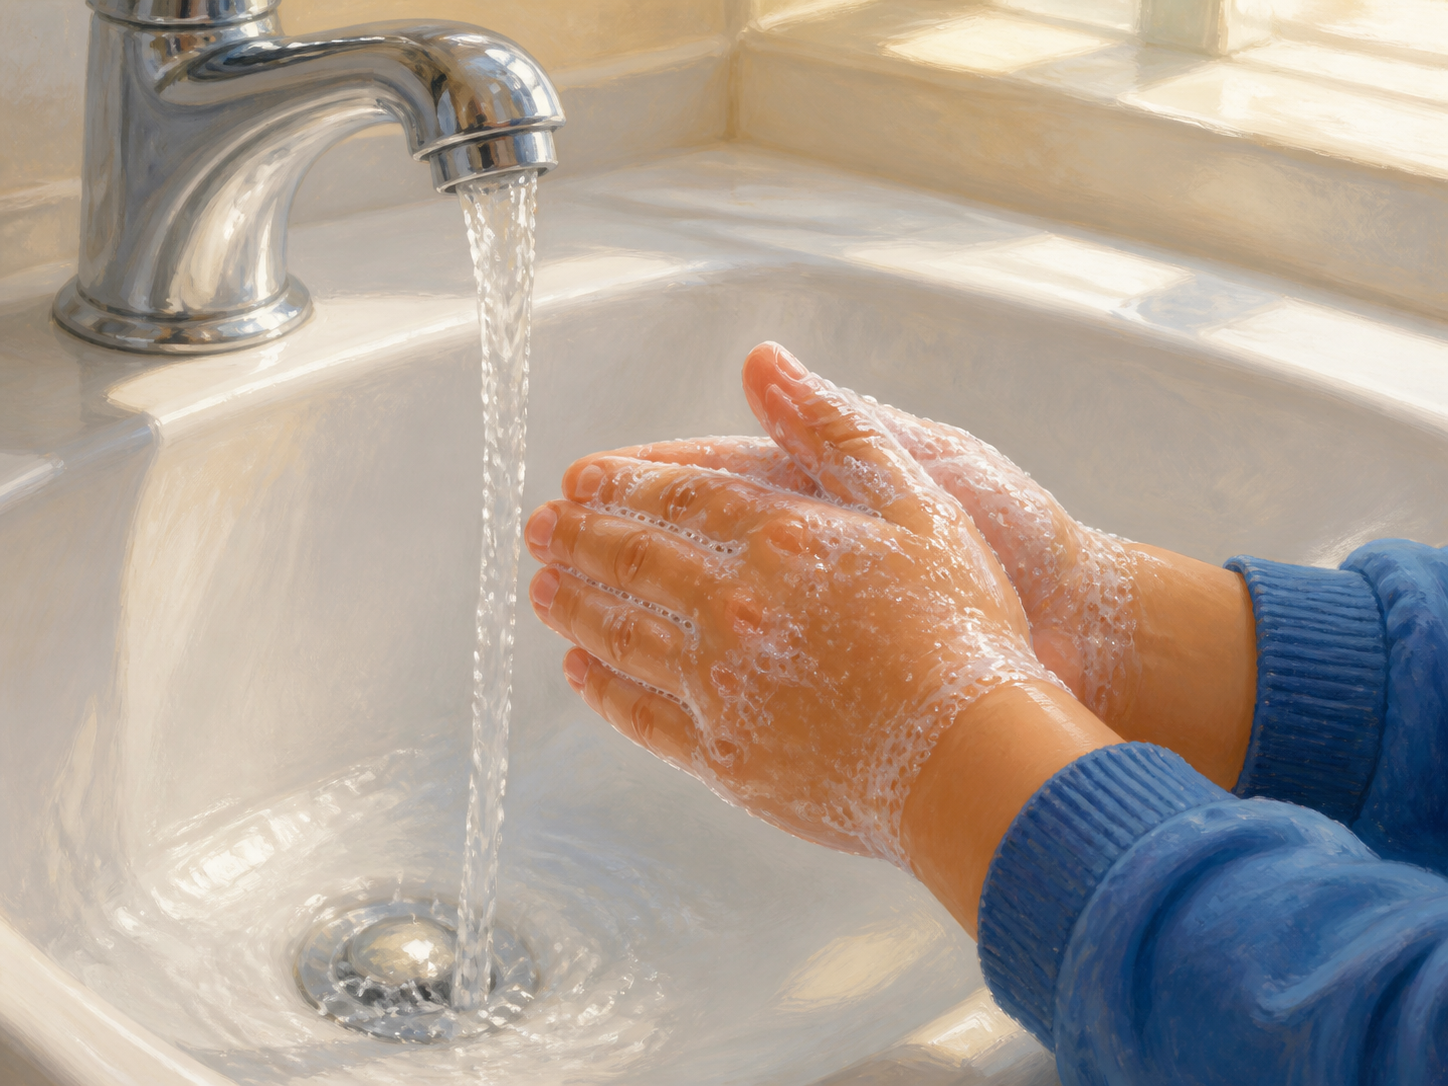
\includegraphics[width=0.58\linewidth]{images/book1/ai/g1-habits-handwashing.png}

{\small Sabun, gosokan, air mengalir: lagu yang paling tidak disukai
\omterm{def:g1:healthy-habits:germs}{kuman} berlangsung selama hitungan pelan sampai dua puluh.}
\end{omfigure}

\begin{example}[Percobaan bubuk kilap]\label{ex:g1:healthy-habits:glitter}
Gosokkan sejumput bubuk kilap pada telapak tanganmu, lalu bersalaman
dengan seorang teman, bukalah sebuah pintu, pungutlah sebatang pensil:
bubuk kilap ada di mana-mana. \omterm{def:g1:healthy-habits:germs}{Kuman} menyebar persis seperti itu, hanya
saja tanpa terlihat. Sekarang cucilah dengan sabun sambil menghitung
sampai $20$ --- bubuk kilapnya hilang, dan begitu pula \omterm{def:g1:healthy-habits:germs}{kumannya}.
\end{example}

\section{Gigi untuk dijaga}

\begin{proposition}[Mengapa gigi harus disikat]\label{prop:g1:healthy-habits:teeth}
Sesudah makan, sisa-sisa makanan tertinggal di gigi. \omterm{def:g1:healthy-habits:germs}{Kuman} di dalam
mulut memakan sisa-sisa itu --- terutama yang manis --- dan perlahan
membuat lubang di gigi, yang terasa sakit. Menyikat menyapu sisanya
sebelum \omterm{def:g1:healthy-habits:germs}{kuman} sempat berpesta.
\end{proposition}
\admitted

\begin{method}[Menyikat gigiku]\label{met:g1:healthy-habits:brush}
\begin{enumerate}
  \item Sikat sesudah sarapan dan sebelum \omterm{prop:g1:healthy-habits:needs}{tidur} --- setiap hari;
  \item sikat setiap sisi setiap gigi: sisi depan, sisi belakang, dan
        sisi atas tempat kamu mengunyah;
  \item jangan tergesa-gesa --- kira-kira selama satu lagu;
  \item gantilah dengan sikat gigi baru ketika \omterm{def:g1:animals-around-us:covering}{bulunya} mengembang.
\end{enumerate}
\end{method}

\begin{remark}[Gigi susu pun penting]\label{rem:g1:healthy-habits:babyteeth}
``Gigi ini toh akan tanggal --- untuk apa disikat?'' Karena gigi itu
masih harus mengunyah untukmu bertahun-tahun lagi, karena lubang
padanya sama sakitnya, dan karena gigi tetap sudah menunggu di
bawahnya dan berhak tiba di dalam mulut yang bersih dan sehat.
\end{remark}

\section{Makan, bergerak, tidur}

\begin{proposition}[Tiga kebutuhan harian]\label{prop:g1:healthy-habits:needs}
Tubuh yang sedang tumbuh membutuhkan, setiap hari:
\begin{enumerate}
  \item \emph{makanan beragam}\index{makanan beragam} --- sedikit dari
        segalanya: sayur dan buah, roti dan biji-bijian, susu dan
        keju, daging atau ikan atau telur, serta air untuk diminum;
        makanan manis hanya sesekali;
  \item \emph{gerak}\index{gerak} --- berlari, memanjat, bersepeda,
        bermain di luar: bergerak membuat otot, tulang dan jantung
        makin kuat;
  \item \emph{tidur}\index{tidur} --- pada malam hari tubuh
        beristirahat, memperbaiki dirinya dan tumbuh; seorang anak
        membutuhkan malam yang panjang, jauh lebih panjang daripada
        orang dewasa.
\end{enumerate}
\end{proposition}
\admitted

\begin{omfigure}
\begin{tikzpicture}
  \draw[thick, omMeth, fill=omMeth!7, rounded corners=6pt]
    (0,0) rectangle (3.6,2.3);
  \draw[thick, omProp, fill=omProp!7, rounded corners=6pt]
    (4.0,0) rectangle (7.6,2.3);
  \draw[thick, omDef, fill=omDef!7, rounded corners=6pt]
    (8.0,0) rectangle (11.6,2.3);
  \node[font=\small\bfseries, omMeth] at (1.8,1.95) {makan beragam};
  \node[font=\small\bfseries, omProp] at (5.8,1.95) {bergerak};
  \node[font=\small\bfseries, omDef] at (9.8,1.95) {tidur};
  \node[font=\small, align=center, text width=3.3cm] at (1.8,0.9)
    {sedikit dari\\ segalanya,\\ air untuk diminum};
  \node[font=\small, align=center, text width=3.3cm] at (5.8,0.9)
    {bermain di luar,\\ berlari, memanjat,\\ setiap hari};
  \node[font=\small, align=center, text width=3.3cm] at (9.8,0.9)
    {malam yang panjang:\\ tubuh memperbaiki\\ diri dan tumbuh};
\end{tikzpicture}

{\small Tiga kebutuhan harian tubuh yang sedang tumbuh. Tidak satu pun
di antara ketiganya dapat menggantikan yang lain.}
\end{omfigure}

\begin{example}[Satu hari yang baik bagi tubuh]\label{ex:g1:healthy-habits:day}
Sarapan dengan buah; tangan dicuci sebelum makan siang; sesore penuh
berlari di taman; gigi disikat sesudah makan malam; lampu dipadamkan
lebih awal dengan sebuah cerita. Tidak ada yang luar biasa --- dan
justru itulah intinya: kesehatan tersusun dari hari-hari biasa seperti
ini.
\end{example}

\begin{remark}[Lelah adalah sebuah pesan]\label{rem:g1:healthy-habits:tired}
Menguap, \omterm{def:g1:the-five-senses:sense}{mata} pedih, uring-uringan tanpa sebab: itulah tubuh yang
berkata ``aku butuh \omterm{prop:g1:healthy-habits:needs}{tidur}''. Mendengarkannya juga sebuah kebiasaan
sehat. Otak yang cukup \omterm{prop:g1:healthy-habits:needs}{tidur} pada pagi hari belajar lebih baik,
bermain lebih baik dan lebih mudah tertawa.
\end{remark}

\section{Latihan}

\begin{exercise}[$\star$]\label{exo:g1:healthy-habits:1}
Apa itu \omterm{def:g1:healthy-habits:germs}{kuman}? Mengapa tangan yang tampak bersih tetap perlu dicuci?
\end{exercise}

\begin{exercise}[$\star$]\label{exo:g1:healthy-habits:2}
Sebutkan tiga saat dalam sehari ketika tangan harus dicuci.
\end{exercise}

\begin{exercise}[$\star$]\label{exo:g1:healthy-habits:3}
Pada \cref{met:g1:healthy-habits:hands}, berapa lama gosokan dengan
sabun seharusnya berlangsung? Sebutkan dua tempat yang mudah terlupa.
\end{exercise}

\begin{exercise}[$\star$]\label{exo:g1:healthy-habits:4}
Mengapa gigi berlubang ketika tidak disikat? Ceritakan kisahnya dengan
\omterm{def:g1:healthy-habits:germs}{kuman} dan sisa makanan.
\end{exercise}

\begin{exercise}[$\star$]\label{exo:g1:healthy-habits:5}
Kapan gigi harus disikat, dan berapa lama waktunya?
\end{exercise}

\begin{exercise}[$\star$]\label{exo:g1:healthy-habits:6}
Sebutkan tiga kebutuhan harian pada \cref{prop:g1:healthy-habits:needs},
dan satu contoh masing-masing dari harimu sendiri.
\end{exercise}

\begin{exercise}[$\star$]\label{exo:g1:healthy-habits:7}
Apa yang dikerjakan tubuh selama \omterm{prop:g1:healthy-habits:needs}{tidur}? Siapa yang membutuhkan malam
lebih panjang, seorang anak atau orang dewasa?
\end{exercise}

\begin{exercise}[$\star$]\label{exo:g1:healthy-habits:8}
Sebutkan dua tanda bahwa tubuh sedang meminta \omterm{prop:g1:healthy-habits:needs}{tidur}.
\end{exercise}

\begin{exercise}[$\star\star$]\label{exo:g1:healthy-habits:9}
Sam berkata: ``Gigi susuku toh akan tanggal, jadi menyikatnya
sia-sia.'' Jawablah ia dengan
\cref{rem:g1:healthy-habits:babyteeth} --- sedikitnya dua alasan.
\end{exercise}

\begin{exercise}[$\star\star$]\label{exo:g1:healthy-habits:10}
Pada percobaan bubuk kilap \cref{ex:g1:healthy-habits:glitter}, bubuk
kilapnya melambangkan apa? Apa yang ditunjukkan percobaan itu tentang
bersalaman --- dan tentang sabun?
\end{exercise}
